\section{Cours}

\subsection{CPU}

Notre CPU se composera ainsi:
\begin{itemize}
\item Des registres
\item Une ALU
\item Une Mémoire
\end{itemize}

\subsubsection{Les registres}
Les registres sont des petites zones de mémoire internes au CPU, il s'agit de la
mémoire la plus rapide de l'ordinateur. Ces registres servent au stockage de
valeurs importantes ou intermédiaires avec lesquelles le processeur est en train
de travailler. Notre CPU travaille sur des mots de 32 bits. Pour rappel un mot
mémoire est une unité de donnée de taille fixe qui représente la plus petite
unité de mémoire que le CPU peut lire, même pour ne lire qu'un seul octet, un
mot mémoire sera lu. Nos registres et instructions auront donc une taille de 32
bits. Par defaut en C\# le mot clef int est sur 32 bits.\\ Un processeur MIPS
possède 32 registres généraux, un PC (Program Counter il contient l'addresse en
mémoire de la prochaine instruction à executer,  il est incrémenté de 4 pour
passer à l'instruction suivante).\\ Deux autres registres HI et LO qui servent à
stocker le resultat d'une division ou multiplication qui serait plus grand qu'un
mot (> 32 bits).
\\\\ Récapitulatif:
\begin{itemize}
  \item 32 registres de 32 bits
  \item 2 registres de 32 bits, HI et LO
  \item PC
\end{itemize}

\subsubsection{ALU}
ALU signifie Arithmetic and Logic Unit, c'est la partie qui va s'occuper
d'effectuer les calculs et les  opérations binaires. C'est dans cet élément que
vous implémenterez par exemple une fonction Add qui prend les pramètres
necessaires, effectue une addition et place le résultat à l'endroit demandé.

\subsection{Environnement}

Nous allons mettre en place un environnement qui devra contenir:
\begin{itemize}
\item Un CPU 
\item Une RAM
\item Une stack (dans la RAM)
\item Un décodeur
\end{itemize}

\subsection{La RAM} Afin d'émuler un environnement, nous allons avoir besoin
d'une RAM, une tableau de byte suffira, cependant il faut prendre une taille
suffisante (64KiB par exemple).\\ Un binaire classique est composé de plusieurs
segments, ce sont des régions regroupant les différents éléments du programme.
Celui qui contient les instructions du programme est le segment .text. Il faudra
le copier dans la RAM à l'addresse 0. Il sera intéressant de garder la taille du
segment copiée en mémoire afin d'implémenter les limites de la stack.

\subsection{Décodeur} Les instructions sont encodés en binaires et peuvent être
stockés dans la mémoire et lu / écrite comme n'importe quelle données.\\ On peut
ainsi les lire et écrire dessus.\\

Une instruction en MIPS possède une taille de 32 octets ou tout simplement 4
bytes et peut se décomposer en différents champs.\\ Chaque champ indique quelque
chose à propos de l'instruction (l'action à effectuer, les paramètres de
l'action, ...).\\

En MIPS il existe 3 types d'instructions :
\begin{itemize}
  \item Les Instructions de type I : qui acceptent des constantes
  \item Les Instructions de type J : L'instruction jump et jal
  \item Les Instructions de type R : Toutes les autres instructions
\end{itemize}

\subsubsection{Les Instructions de type R}

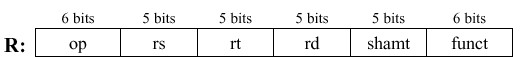
\includegraphics[width = 12.11cm]{R-type.jpg}
~ \\ ~ \\
Les Instructions de type R se décomposent selon le shéma ci-dessus.  Le champ op
correspond à l'operation à effectuer. Dans le cas d'une instruction de type R ce
champ est mis à 0 et il faut regarder le champ funct pour avoir l'instruction à
effectuer.\\

Rs, Rt et Rd correspondent respectivement au registre source, target et
destination. Ceux-ci sont utilisés lors des opérations registre vers registre.
Enfin shamt est le champ utilisé lors d'un shift.

\subsubsection{Les Instructions de type I}

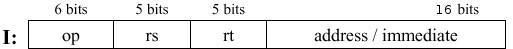
\includegraphics[width = 12.11cm]{I-type.jpg}
~ \\ ~ \\
Les Instructions de type I se décomposent selon le shéma ci-dessus. Le champ op
correspond à l'operation à effectuer. Rs et Rt correspondent respectivement au
registre source et target.

Enfin, address / immediate correspond à une constante (un entier ou une addresse
dans la memoire) sur laquelle on veut effectuer des actions.

\subsubsection{Les Instructions de type J}

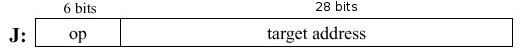
\includegraphics[width = 12.11cm]{J-type.jpg}
~ \\ ~ \\
Les Instructions de type J se décomposent selon le shéma ci-dessus. Le champ op
correspond à l'operation à effectuer.

Celles-ci sont au nombre de deux :
\begin{itemize}
  \item Jmp : permet de sauter dans la memoire. L'adresse est calculée de la
    manière suivante : New PC = addresse * 4
  \item Jal : Effectue la meme action que Jmp mais sauvegarde l'addresse avant
    de sauter sur le stack.
\end{itemize}

A noter que étant donné la taille de notre mémoire pour ce Tp qui est de 64 kib,
au lieu de prendre 28 bits nous nous contenterons de 16.


\subsection{La stack}
Les registres étant limités, il faut pouvoir stocker les données dans la RAM. On
utilise une pile afin de pouvoir empiler des éléments et les dépiler lorsque
l'on a fini de travailler avec.\\ Par exemple lorsque l'on appelle une fonction,
le PC est modifié pour pointer sur la première instruction de celle-ci, donc on
sauvegarde l'ancienne valeur de PC sur la pile. On aura donc une succession de
valeurs de PC empilées sur la stack et lorsque les différentes fonctions feront
des return, on dépilera les valeurs afin de restaurer le PC.\\ Il y a plusieurs
manières d'implémenter la stack, soit en la faisant débuter à l'addresse la plus
haute et en la faisant grandir vers les addresses basses, soit en la faisant
débuter juste après la fin du segment .text et en la faisant grandir jusqu'a la
limite de la RAM.

\section {Les fichiers} Les programmes de test que nous vous donnerons (qui
contiendront le segment .text) devront être copiés en RAM, mais avant il faudra
les lire.\\ Les différents flux de données (fichiers, réseau, etc...) sont
accessibles via une classe de base Stream. Plusieurs classes sont dérivées de
celle-ci afin de représenter plus précisément un usage: FileStream,
NetworkStream, ...\\ Pour la manipulation de fichiers, le namespace sera
System.IO et nous allons nous intéresser à la classe static File de celui-ci qui
contient une methode Exists:
\begin{code}
  public static bool Exists(string path)
\end{code}

Cette fonction parle d'elle-même: elle retourne un booléen qui indique si le
fichier donné en paramètre existe.

Nous allons maintenant récupérer un FileStream qui nous permettra de lire le
contenu de notre fichier.\\ Toujours dans File, nous avons une methode Open:
\begin{code}
  public static FileStream Open(string path, FileMode mode)
\end{code}

Le mode permet de définir le comportement à adopter vis à vis du fichier
(l'ouvrir, le créer, l'écraser, ajouter à la fin, ...).\\ Celui qui nous
interesse pour une simple lecture est FileMode.Open\\ Afin de manipuler un
Stream, plusieurs classes existent en fonction du type de donnée, la différence
sera dans les methodes fournies qui seront plus adaptées pour le type en
question. Nous allons lire des données binaires, nous utiliserons donc
BinaryReader.

\begin{code}
public BinaryReader(Stream input)
\end{code}

Le constructeur prend un stream en paramètre, FileStream étant une classe
dérivée de celle-ci, nous pouvons tout à fait lui donner un FileStream en
paramètre.\\ Pour lire le fichier avec notre BinaryReader nous utiliserons une
methode de celui-ci:

\begin{code}
public virtual byte[] ReadBytes(int count)
\end{code}

Le mot clef virtual n'a aucune importance pour nous. Cette methode prend en
paramètre le nombre de bytes à lire dans le fichier puis nous les renvoie sous
forme d'un tableau.

Vous pouvez connaitre la taille d'un fichier en utilisant le champ Length d'un
Stream (sur fichier uniquement !), Regardez les différents champs du
BinaryReader pour retrouver le Stream d'origine.

\newpage
